\documentclass{beamer}
\usepackage{lsfolien}
\usepackage[english]{babel}
\usepackage[utf8]{inputenc}

\myfootline{System Modelling and Semantic Web -- Spring 2021}{Hans-Gert Gräbe}

\newcommand{\ueberschrift}[1]{\begin{center}\bf #1\end{center}}

\title{Modelling Sustainable Systems\\ and Semantic Web\\[6pt]
  Internet Basics
  \vskip1em}

\subtitle{Lecture in the Module 10-202-2309\\ for Master Computer Science}

\author{Prof. Dr. Hans-Gert Gräbe\\
\url{http://www.informatik.uni-leipzig.de/~graebe}}

\date{June 2021}
\begin{document}

{\setbeamertemplate{footline}{}
\begin{frame}
  \titlepage
\end{frame}}

\section{Internet Basics}
\begin{frame}{Internet Basics}
In the following, we will use the concept of \emph{role} as partial identity
as basis when looking at the technical basics of the operation of digital
identities (more precisely: \emph{as} digital identities).

\begin{itemize}
\item On the internet descriptions are exchanged.
\begin{itemize}
\item[] Images, for example, are also descriptions that instruct the computer
  how to render the image.
\end{itemize}
\item Descriptions are exchanged between computers by breaking them down into
  packets of a given structure and size.
\end{itemize}

\ueberschrift{Packet transmission on the internet, the OSI 7-layer model}
\begin{itemize}
\item \url{http://de.wikipedia.org/wiki/OSI-Modell}
\item Layers and protocols
\item Protocols and language
\end{itemize}
\end{frame}
\begin{frame}{Internet Basics. The OSI Layer Model}
  \begin{center}\small
    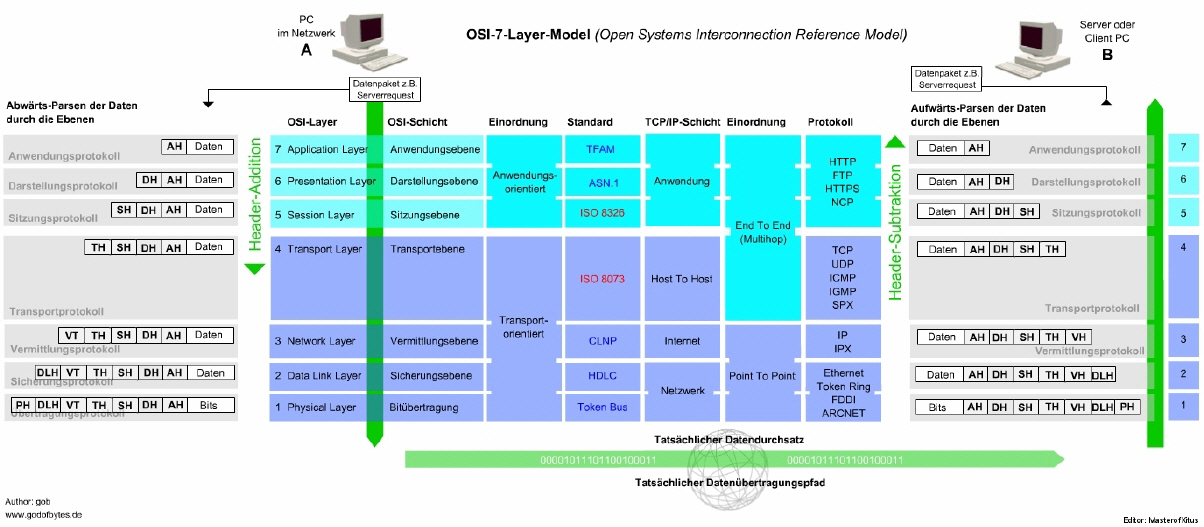
\includegraphics[width=\textwidth]{Rqw330.jpg}\\
    Source: Wikipedia, \url{http://prima-it.de/images/osi7layermodell.jpg} 
  \end{center}
\end{frame}
\begin{frame}{Internet Basics. The OSI Layer Model}
  \begin{center}\small
    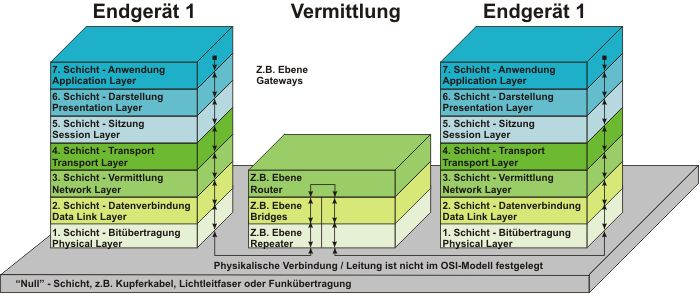
\includegraphics[width=\textwidth]{HhBzfw.jpg}\\
    Source: \url{http://www.hbernstaedt.de/knowhow/ether/osi.jpg}
  \end{center}
\end{frame}
\begin{frame}{Internet Basics. How It Works}
Texts consist of characters (letters, numbers, etc.)
\begin{itemize}
\item Bits and Bytes.
\item Reduction to standardised bit sequences and thus numbers.
  \begin{itemize}
  \item First permanent alphabet: ASCII (7 bits) = 0..127
  \item 0..31 -- control characters.
  \item 32..127 -- numbers and letters of the English alphabet.
  \end{itemize}
\item Several waves of standardisation for further alphabets and character
  systems (latin-1, Windows character set).
\item Need to agree $\to$ Unicode.
  \begin{itemize}
  \item Efforts begin around 1988.
  \item First standard in 1991 contained 216 = 65\,536 characters.
  \end{itemize}
\end{itemize}
\end{frame}
\begin{frame}{Internet Basics. Unicode} 
International standard in which (in the long term) a digital code is defined
for every meaningful character or text element of all known writing cultures
and character systems in order to standardise the exchange of textual
information worldwide.

\begin{itemize}
\item Unicode is constantly being supplemented with characters from other.
  writing systems.
  \begin{itemize}
  \item Hexadecimal representation, e.g. U+01FA (2 bytes).
  \end{itemize}
\item UTF-8 as an evolving de-facto standard.
  \begin{itemize}
  \item Encoding of characters in up to 4 bytes (variable length).
  \item Encoding of ASCII characters in 1 byte.
  \end{itemize}
\end{itemize}
\end{frame}
\begin{frame}{Internet Basics. Data transmission}

\begin{itemize}
\item Serial transmission as a bit sequence, for human-readable purposes
  usually represented in the octal or (more frequently) hexadecimal system
  (base 16) (x1FA = 0001.1111.1010).
\item Bit stream is divided into packets of constant length and sent off with
  sender/receiver information (routing).
\item Packets are forwarded from computer to computer until they reach their
  recipient.
\item Integrity check with a hash function.
\item Receiver reassembles the bit stream from the packets.
\item Standardised protocols are used so that this is transparent for the
  user.
\end{itemize}
\end{frame}
\begin{frame}{Internet Basics}
  \begin{center}
    \begin{tabular}{|c|c|c|}\hline
      \textbf{Function} & \textbf{OSI Layer} & \textbf{Protocols}\\\hline
      &Anwendungsschicht & HTTP\\
      Anwendung & Darstellungsschicht & HTTPS\\
      &Sitzungsschicht & SSH\\\hline
      Netzübertragung & Transportschicht & TCP/IP \\
      & Vermittlungsschicht & SSH/SSL \\\hline 
      Netzzugang & Sicherungsschicht & WLAN, PPP \\
      &Übertragungsschicht & Ethernet \\\hline
    \end{tabular}
  \end{center}
\end{frame}

\section{Computer Networks}
\begin{frame}{What Computers Talk About with each Other}
\emph{Example:} \url{http://www.inspirata.de} 
\begin{itemize}
\item Web pages are composed of different parts that can come from different
  sources.
\item Parts in different languages (HTML, graphic formats, programme code,
  ...), the languages determine the form of presentation.
\item Rendering web pages therefore (usually) means bringing together
  heterogeneous information from different sources.
\end{itemize}
\end{frame}
\begin{frame}{Internet as World of Fictions}
Two dimensions of language: description and instruction.
\begin{itemize}
\item HTML (HyperText Markup Language) -- the language of the internet? 
\item HTTP -- HyperText Transfer Protocol.
\end{itemize}
The Internet as a \textbf{World of Iterated Fictions}: 
\begin{itemize}
\item Interpretation of modulated electromagnetic waves as sequences of
  0-1-bitstreams. 
\item Intermediate: frames (OSI level 2), packets (OSI level 3)
\item Interpretation of bit streams as "digital content".
\item Interpretation of digital content as text, pictures, code etc. for
  rendering. 
\item Interpretation of rendered content by humans.
\end{itemize}
\end{frame}
\begin{frame}{On the Assignment of Digital Identities}

\emph{Digital identity} = \emph{authenticated} and \emph{authorised} within a
session real-world civic subject, who performs actions in the digital universe
for a limited period of time.

Such digital identities do not fall from the sky, but must be embedded in the
civil legal order for the purpose of private assignment of the consequences of
actions.
\begin{itemize}
\item Market economy: Regulatory framework and contractual arrangements in a
  hierarchical socio-technical system.
\end{itemize}
Who authenticates and authorises? 
\begin{itemize}
\item Computers, computer networks, computer names.
\item Registrar, provider, host.
\end{itemize}
\end{frame}
\begin{frame}{Computer and Computer Names}
\begin{center}\small
  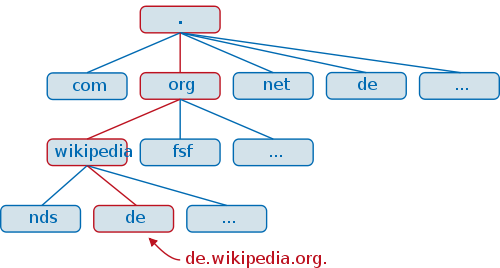
\includegraphics[width=.8\textwidth]{f8L17R.png}
\end{center}
\begin{itemize}
\item IPv4 (32 bit) and IPv6 (128 bit) -- \texttt{ping} and \texttt{ifconfig}
\item On the structure of computer names, domain names and top level domains.
\item Converting names into addresses -- the Domain Name Service System.
\end{itemize}\vskip2em
\end{frame}
\begin{frame}{Registrar, Provider, Host}
\begin{itemize}
\item \textbf{Registrar:} Administrator of computer names
  \begin{itemize}
  \item Denic.de -- The administrator of the TLD .de is DENIC e.G.
  \item Citation Imprint: Registered under No. 770 in the Register of
    Cooperatives, Frankfurt/Main Local Court.
  \item Notes on the legal form
  \item URZ administers \texttt{uni-leipzig.de} and subdomains
  \end{itemize}
\item Which domain names?
  \begin{itemize}
  \item Ownership of a domain as a legal title
  \item Computer names as a commodity:
    \url{https://sedo.com/de/wissen/markt-trends/}
  \end{itemize}
\item \textbf{Provider:} Maintains computers with IP addresses
  (\textbf{Hosts}) and takes care of converting domain names into IP addresses
  as well as forwarding (routing) data packets.
\end{itemize}
\end{frame}
\begin{frame}{Allocation of IP Addresses}\small
\begin{itemize}
\item IP addresses are allocated hierarchically: Users get IP addresses from
  the ISP (internet service provider), ISPs from a local Internet registry
  (LIR) or National Internet Registry (NIR) or Regional Internet Registry (RIR
  -- RIPE NCC for Europe, the Middle East, and Central Asia) and these from
  the Internet Assigned Numbers Authority (IANA).
\item IANA is a department of ICANN responsible for coordinating some of the
  key elements that keep the Internet running smoothly. Whilst the Internet is
  … free from central coordination, there is a technical need for some key
  parts of the Internet to be globally coordinated, and this coordination role
  is undertaken by IANA. IANA is one of the Internet's oldest institutions,
  with its activities dating back to the 1970s. $\to$
  \url{https://www.iana.org/numbers}
\item \emph{Question:} Can I buy IP addresses from the RIPE NCC? 

  \emph{Answer:} No. Internet number resources are a shared public resource
  and do not have a value. Members are charged fees based on the services that
  they receive from the RIPE NCC.
\end{itemize}
\end{frame}
\end{document}
